\chapter{Introduction}
\section{What is Steganography}
Steganography is the practise of concealing information within a medium, originating from the Greek words "steganos" (covered) and "graphial" (writing). This entails concealing the data so that only the intended recipient is aware of its presence. While archaic methods entailed concealing data on the backs of wax, writing tables, or even rabbit bellies, modern methods often involve transferring data in the form of text, images, video, and audio across numerous mediums. Multimedia items are frequently employed as cover sources to conceal sensitive data during transmission. Steganography's goal is to permit invisible communication while guaranteeing confidentiality between communicative parties.
We intend to discuss several security and data concealment techniques that can be utilised in steganography, such as LSB and PVD, in this study. We will investigate the strategies' strengths and drawbacks, as well as their applicability in various circumstances. Our goal is to provide a thorough understanding of steganography and its potential applications. Readers will have a better knowledge of steganography and its function in facilitating secure communication by the end of this paper.
\begin{figure}[ht!]
\centering
\frame{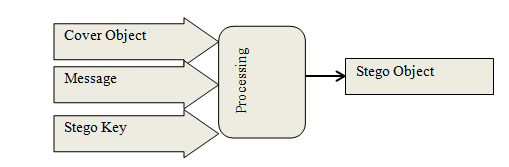
\includegraphics[width=35em, height=38mm]{figures/Pictures/What is steganograghy.png}}
\caption{Steganography Action. Adapted from \cite{article2}}
\end{figure}
\section{Process}
\textbf{The steganography process involves several steps:}
\begin{enumerate}
\item Select and convert the secret data into a binary format.
\item Choose a cover object, such as an image or audio file.
\item Embed the secret data into the cover object using a steganographic algorithm.
\item Create a new file, known as the stego-object, which appears identical to the original cover object but contains the hidden secret data.
\item Transmit the stego-object over a chosen medium to the intended recipient.
\item Extract the secret data using a reverse steganographic algorithm.
\end{enumerate}

By following these steps, steganography allows for the secure and discreet transmission of confidential information.
\section{History}
Steganography has an interesting history that dates back to ancient Greece. It has been used to disguise messages in a variety of methods, including ink and milk, as well as digital images, audio, and video files. Despite its growth, steganography's primary purpose remains the same: to keep information secret. This centuries-old strategy is still important in current communication.

\section{Image steganography}
Image steganography is a technique for concealing sensitive information within digital photographs. The secret information is encoded into the image pixels using a steganographic technique, resulting in a new image that appears identical to the original, known as the stego-image. The stego-image can be conveyed to the receiver via a specified medium, and the secret information can be extracted using a reverse steganographic technique. Despite the fact that image steganography is a common technique due to the popularity of digital photographs, it can be detected through statistical analysis or visual inspection.

